% =============================================================================
%  TDK-dolgozat (Budapesti Corvinus Egyetem, 2026/27) — Vonalszintű nyílt
%  Markov-hálózat a budapesti közösségi közlekedés utasáramlására
%  Formai előírások: Times New Roman 12, 1,5-es sorköz, sorkizárt, 2,5 cm margó.
%  Minden szám a scripts/tdk_analysis.py futtatásából származik
%  (BKK GTFS 2572.20260604, szolgáltatási nap: 2026. június 9., kedd).
% =============================================================================
\documentclass[12pt,a4paper]{article}

% --- Kódolás és nyelv ---
\usepackage[T1]{fontenc}
\usepackage[utf8]{inputenc}
\usepackage[magyar]{babel}

% --- Tipográfia ---
\usepackage{mathptmx}          % Times New Roman (szöveg és matematika)
\usepackage{microtype}

% --- Matematika ---
\usepackage{amsmath}
\usepackage{amssymb}
\usepackage{amsthm}
\usepackage{bm}

\newtheorem{tetel}{Tétel}[section]
\newtheorem{lemma}[tetel]{Lemma}
\newtheorem{kovetkezmeny}[tetel]{Következmény}
\newtheorem{allitas}[tetel]{Állítás}
\theoremstyle{definition}
\newtheorem{definicio}[tetel]{Definíció}
\newtheorem{felteves}[tetel]{Feltevés}
\theoremstyle{remark}
\newtheorem{megjegyzes}[tetel]{Megjegyzés}

% --- Ábrák és táblázatok ---
\usepackage{graphicx}
\usepackage{float}
\usepackage[section]{placeins}
\usepackage{booktabs}
\usepackage{caption}
\captionsetup{font=small,labelfont=bf,labelsep=period}
\captionsetup[figure]{name=ábra}
\captionsetup[table]{name=táblázat}

% --- Linkek, oldal ---
\usepackage[hidelinks,unicode]{hyperref}
\usepackage[margin=2.5cm]{geometry}
\usepackage{setspace}
\onehalfspacing
\usepackage{enumitem}
\setlist{itemsep=2pt,topsep=4pt}
\usepackage{xcolor}
\usepackage{url}
\usepackage[round,authoryear]{natbib}
\usepackage{csquotes}

% --- A futtatásból származó számok (scripts/tdk_tex_numbers.py generálja) ---
% generated by scripts/tdk_tex_numbers.py -- do not edit
\newcommand{\FEEDVER}{2572.20260604}
\newcommand{\NTRIPS}{39\,662}
\newcommand{\NUNION}{96\,033}
\newcommand{\INFL}{2{,}42}
\newcommand{\NHUBS}{2\,372}
\newcommand{\NSEGS}{11\,341}
\newcommand{\NSTATES}{13\,713}
\newcommand{\NTRIPSEG}{104\,004}
\newcommand{\MEDCVSQ}{0{,}019}
\newcommand{\SHARECVLOW}{90}
\newcommand{\MEDCVSQMETRO}{0{,}004}
\newcommand{\MEDTAU}{60}
\newcommand{\MEDDIST}{387}
\newcommand{\NSINGLE}{581}
\newcommand{\SEGBUS}{9\,238}
\newcommand{\DEPBUS}{72\,518}
\newcommand{\SEGTRAM}{1\,389}
\newcommand{\DEPTRAM}{19\,042}
\newcommand{\SEGTROLLEY}{446}
\newcommand{\DEPTROLLEY}{6\,634}
\newcommand{\SEGMETRO}{96}
\newcommand{\DEPMETRO}{4\,412}
\newcommand{\SEGHEV}{170}
\newcommand{\DEPHEV}{1\,390}
\newcommand{\SEGFERRY}{2}
\newcommand{\DEPFERRY}{8}
\newcommand{\THETAF}{1{,}92}
\newcommand{\BOARDPH}{400\,000}
\newcommand{\JOURNPH}{280\,005}
\newcommand{\LEGS}{1{,}43}
\newcommand{\INSYS}{68\,189}
\newcommand{\WAITING}{11\,328}
\newcommand{\RIDING}{56\,861}
\newcommand{\WAITSHARE}{16{,}6}
\newcommand{\EJOURNEY}{14{,}6}
\newcommand{\WAITBOARD}{1{,}70}
\newcommand{\WAITBOARDOLD}{3{,}17}
\newcommand{\RIDELEG}{8{,}5}
\newcommand{\MAXSEGFLOW}{1\,454}
\newcommand{\MAXHUBBOARD}{4\,081}
\newcommand{\MCN}{200\,000}
\newcommand{\MCSEC}{0{,}42}
\newcommand{\MCMEAN}{14{,}62}
\newcommand{\MCSE}{0{,}031}
\newcommand{\MCRELERR}{0{,}04}
\newcommand{\MCOCCERR}{8{,}4}
\newcommand{\EJOURNEYTWO}{14{,}61}
\newcommand{\JQFIFTY}{10{,}6}
\newcommand{\JQNINETY}{32{,}0}
\newcommand{\TFIFTY}{9}
\newcommand{\TNINETY}{32}
\newcommand{\TNINETYFIVE}{42}
\newcommand{\TRELAX}{173}
\newcommand{\SLAMZEROJ}{14{,}4}
\newcommand{\SLAMSIXTYJ}{15{,}3}
\newcommand{\SLAMSIXTYW}{23{,}2}
\newcommand{\SLAMZEROW}{14{,}5}
\newcommand{\SLAMSIXTYRHO}{0{,}947}
\newcommand{\SDLOW}{12{,}4}
\newcommand{\SDHIGH}{17{,}1}
\newcommand{\SPLOW}{12{,}7}
\newcommand{\SPHIGH}{17{,}1}
\newcommand{\SMINRHOHUB}{0{,}998}
\newcommand{\SMINRHOSEG}{0{,}947}
\newcommand{\EZERO}{4{,}84}
\newcommand{\EHARM}{34{,}4}
\newcommand{\RESSEC}{11}
\newcommand{\RHOTHRU}{0{,}73}
\newcommand{\RHOCF}{0{,}77}
\newcommand{\FAILNAMEA}{Puskás Ferenc Stadion}
\newcommand{\FAILNETA}{3{,}8}
\newcommand{\FAILNAMEB}{Keleti pályaudvar}
\newcommand{\FAILNETB}{3{,}5}
\newcommand{\FAILNAMEC}{Örs vezér tere}
\newcommand{\FAILNETC}{3{,}4}
\newcommand{\MSBMETRO}{6{,}5}
\newcommand{\MSKMETRO}{6{,}8}
\newcommand{\MSBBUS}{66{,}1}
\newcommand{\MSKBUS}{66{,}3}
\newcommand{\MSBTRAM}{19{,}9}
\newcommand{\MSKTRAM}{19{,}9}
\newcommand{\MSBTROLLEY}{5{,}9}
\newcommand{\MSKTROLLEY}{4{,}7}
\newcommand{\MSBHEV}{1{,}7}
\newcommand{\MSKHEV}{2{,}2}


\hyphenation{va-ló-szí-nű-sé-gi ge-ne-rá-tor-mát-rix cso-mó-pont cso-mó-pon-tok}

\newcommand{\E}{\mathbb{E}}
\newcommand{\Var}{\operatorname{Var}}
\newcommand{\one}{\mathbf{1}}
\newcommand{\Hs}{\mathcal{H}}
\newcommand{\Ss}{\mathcal{S}}
\newcommand{\Xs}{\mathcal{X}}

\begin{document}
\renewcommand{\abstractname}{Összefoglaló}

% ------------------------------------------------------------------ címlap --
\begin{titlepage}
  \centering
  {\large Budapesti Corvinus Egyetem}\\[2pt]
  {Tudományos Diákköri Konferencia, 2026.~őszi félév}\\[2pt]
  {[Szekció neve]}\\[3.5cm]
  {\LARGE\bfseries Vonalszintű nyílt Markov-hálózat\\[4pt]
   a budapesti közösségi közlekedés\\[4pt] utasáramlására\par}
  \vspace{0.8cm}
  {\large Egzakt megoldás és sérülékenységi elemzés a BKK GTFS-adatai alapján\par}
  \vfill
  \begin{flushright}
    \textbf{Szerző:} Molnár Marcell, [szak, évfolyam]\\
    \textbf{Témavezető:} [Témavezető neve, beosztása, tanszéke]
  \end{flushright}
  \vspace{1.5cm}
  Budapest, 2026
\end{titlepage}

% -------------------------------------------------------------- összefoglaló --
\begin{abstract}
\noindent
A dolgozat a BKK nyilvános GTFS-menetrendjéből folytonos idejű Markov-modellt
épít a budapesti közösségi közlekedés utasáramlására. Az utas állapota vagy
egy átszállási csomópontban való várakozás, vagy egy vonalszakaszon való
utazás, így a járművön maradás és a menetidő a dinamika része. A beszállási
rátát a menetrendi követési idők első két momentumához illesztjük, ami
szabályos menetrendnél a gyakoriság kétszerese. A viszonylatválasztást a
minimális relatív entrópia elvéből vezetjük le, és megmutatjuk, hogy a
Poisson-folyamatok ritkítása ezt pontosan megvalósítja. Független
Poisson-beáramlás mellett az állapotok foglaltsága minden időpontban független
Poisson-eloszlású, az utazási idő fázistípusú, így a modell egyetlen ritka
lineáris egyenletrendszerrel egzaktul megoldható, a sztochasztikus szimuláció
pedig csak ellenőrzésre kell. A 2026.~június 9-i reggeli csúcsra
alkalmazva a modell a budapesti átszállóközpontok ismert sorrendjét adja, az
igényekkel súlyozott hatékonyságon alapuló sérülékenységi elemzés pedig
megmutatja, hogy egy csomópont hálózati szerepe nem azonos a forgalmával. Az
eredményeket valós Budapest-térképen mutatjuk be.

\medskip\noindent
\textbf{Kulcsszavak:} folytonos idejű Markov-lánc, nyílt sorbanállási hálózat,
fázistípusú eloszlás, minimális relatív entrópia, GTFS, hálózati sérülékenység.
\end{abstract}

\newpage
\tableofcontents
\newpage

% =============================================================================
\section{Bevezetés}
\label{sec:bev}

A BKK járatain munkanaponként átlagosan $3{,}4$~millió felszállás történik
\citep{bkk2024}. A térben és időben felbontott utasforgalom (hány utas vár egy
csomópontban, mekkora a terhelés egy vonalszakaszon) azonban nyilvános
adatokból közvetlenül nem figyelhető meg: a menetrend GTFS formátumban
szabadon elérhető, az utasszámláló és jegyadatok viszont nem. Ebből a helyzetből
természetesen adódik egy olyan valószínűségi modell, amely a menetrend által
meghatározott kínálatból és néhány átlátható feltevésből vezeti le az
áramlásokat. Egy ilyen modell nem helyettesíti a mért utasszámokat, de
kiindulópontot ad az adatasszimilációhoz, és alkalmas a hálózat szerkezeti
sérülékenységének vizsgálatára.

\paragraph{Kutatási kérdés.}
Felépíthető-e kizárólag nyilvános menetrendi adatokból olyan utasáramlási
modell, amely (i)~valószínűség-elméletileg következetes (helyes
mértékegységek, állomány és áramlás megkülönböztetése, a járművön maradás
modellezése), (ii)~a teljes budapesti hálózaton egzaktul megoldható, és
(iii)~értelmezhető választ ad arra, mely csomópontok kiesése rontja leginkább
a hálózat teljesítményét?

\paragraph{Hozzájárulások.}
\begin{enumerate}[label=(\roman*)]
  \item Vonalszintű nyílt Markov-hálózat a budapesti hálózatra, amelyben az
    utas a járművön marad, amíg le nem száll; a várakozási ráta a
    követési idő első két momentumához illeszkedik.
  \item A viszonylatválasztás levezetése a minimális relatív entrópia elvéből,
    és annak bizonyítása, hogy a Poisson-ritkítás ezt pontosan megvalósítja.
  \item Egzakt megoldás: a foglaltságok minden időpontban független
    Poisson-eloszlásúak, az utazási idő fázistípusú eloszlású.
  \item Igényekkel súlyozott, várható időkön alapuló sérülékenységi mutató,
    amely elkülöníti egy csomópont bezárásának közvetlen és hálózati hatását.
  \item Nyílt, reprodukálható Python-megvalósítás, amely a dolgozat minden számát
    egyetlen futtatással előállítja.
\end{enumerate}

A dolgozat felépítése: a \ref{sec:irodalom}.~fejezet a kapcsolódó irodalmat
tekinti át, a \ref{sec:adat}.~fejezet az adatokat és a hálózat felépítését,
a \ref{sec:modell}.~fejezet a modellt, a \ref{sec:megoldas}.~fejezet az egzakt
megoldást, a \ref{sec:serules}.~fejezet a sérülékenységi mutatót ismerteti. Az
eredményeket a \ref{sec:eredmeny}., a korlátokat a \ref{sec:korlat}.~fejezet
tárgyalja.

% =============================================================================
\section{Kapcsolódó irodalom}
\label{sec:irodalom}

\paragraph{Entrópia és forgalomeloszlás.}
\citet{wilson1969} a gravitációs forgalomeloszlási modellt az entrópia
maximalizálásából vezette le: adott átlagos költség mellett a legkevésbé
\enquote{elkötelezett} eloszlás exponenciálisan bünteti a költséget.
\citet{snickars1977} ezt a priori súlyokkal általánosította (minimális
információ, illetve relatív entrópia elve); a dolgozatban ezt az
általánosítást alkalmazzuk a viszonylatválasztásra, ahol az a~priori súlyt a
menetrendi gyakoriság adja.

\paragraph{Gyakoriságalapú ráterhelés.}
A közös vonalak problémájában \citep{chriqui1975} az utas a vonzó viszonylatok
közül az elsőként érkező járműre száll fel, így az egyes vonalak választási
valószínűsége a gyakoriságukkal arányos. \citet{spiess1989} optimális
stratégiákra épülő ráterhelési modellje ma is a menetrendalapú tervezés
alapja. Modellünk beszállási mechanizmusa ennek valószínűségi, folytonos idejű
megfelelője.

\paragraph{Várakozási idő.}
Véletlenszerűen érkező utas esetén a várakozás a követési idő maradék
élettartama, amelynek várható értéke a követési idő négyzetes relatív
szórásától függ (\enquote{inspection paradox}, \citealp{larson1981}). Ebből
következik, hogy a gyakorisággal egyenlő rátájú exponenciális várakozás
szabályos menetrendnél kétszeresére becsüli a várakozást, amit a
\ref{sec:modell}.~fejezetben momentumillesztéssel korrigálunk.

\paragraph{Markov-hálózatok és fázistípusú eloszlások.}
\citet{jackson1957} nyílt sorbanállási hálózatai óta ismert, hogy Markov-típusú
útvonalválasztás mellett a stacionárius eloszlás szorzat alakú. Végtelen sok
kiszolgálós csomópontok és Poisson-beáramlás esetén a foglaltságok független
Poisson-eloszlásúak, ami a Poisson-folyamatok jelöléstételéből következik
\citep{kingman1993}. Az elnyelődésig eltelt idő fázistípusú eloszlású
\citep{neuts1981}. Kémiai reakcióhálózatokban \citet{jahnke2007} megmutatta,
hogy elsőrendű reakciók esetén a mesteregyenlet megoldása Poisson- és
multinomiális eloszlások konvolúciója. Emiatt a \citet{gillespie1977}-féle
pontos szimulációra ilyen rendszerekben csak ellenőrzésként van szükség.

\paragraph{Hálózati sérülékenység.}
\citet{latora2001} hatékonysági mutatója a csúcspárok közötti legrövidebb
utak reciprokának átlaga, amely széteső gráfra is értelmezett.
Közösségi közlekedési hálózatokra \citet{cats2014} dinamikus, utasforgalommal
súlyozott sérülékenységi elemzést javasolt. Mi a hatékonyságot igényekkel
súlyozzuk, a legrövidebb utakat pedig várható várakozási és menetidőkből
számoljuk.

% =============================================================================
\section{Adatok és hálózat}
\label{sec:adat}

\subsection{A rögzített menetrend}

A BKK GTFS-adatait a MobilityData hivatalos tükréről töltöttük le; a
változat azonosítója \texttt{\FEEDVER}, érvényessége 2026.~június~2.
és július~4. közötti. Szolgáltatási napnak a 2026.~június~9-i keddet
választottuk (tanítási nap, ünnepnap nélkül), az elemzési ablak a
07:00--09:00 közötti reggeli csúcs. Az aznap közlekedő \NTRIPS{} menet hat
közlekedési módot fed le.

\paragraph{Két adatkezelési buktató.}
(1)~A menetrend nem tartalmaz \texttt{calendar.txt} fájlt; a szolgáltatási
napokat kizárólag a \texttt{calendar\_dates.txt} kivételei határozzák meg. Ha
a szűrés a hét napja szerint történik (\enquote{minden kedd}), az eredmény a
menetrendi időszak összes keddjének szolgáltatásait egyesíti: \NUNION{}
menetet a június~9-i \NTRIPS{} helyett, ami minden gyakoriságot
\INFL-szeresére növelne. Ezért egyetlen konkrét dátumra szűrünk. (2)~A
jelenlegi menetrend a trolibuszt a szabványos $11$-es, a HÉV-et a kiterjesztett
$109$-es \texttt{route\_type} kóddal jelöli; a régebbi menetrendekben
használt $800$-as és $2$-es kódokra épülő szűrés mindkét módot elveszítené.

\subsection{Csomópontok és vonalszakaszok}

\begin{definicio}[Csomópont]
A peronokat először a \texttt{parent\_station} mező szerinti állomásukhoz
rendeljük. Két állomás egy \emph{csomópontba} tartozik, ha nevük az
\enquote{M}, \enquote{H}, \enquote{M+H} átszállási utótagok elhagyása után
megegyezik, és legfeljebb $400$~m-re vannak egymástól (egyszerű láncszerkesztés,
\emph{single linkage}). A csomópontok halmazát $\Hs$ jelöli.
\end{definicio}

Így kerül egy csomópontba például a Deák Ferenc téri metróállomás és a felszíni
\enquote{Deák Ferenc tér M} buszmegálló, ami nélkül a módok közötti átszállás
nem modellezhető.

\begin{definicio}[Vonalszakasz]
Az $s=(\ell,i,j)$ vonalszakasz az $\ell$ viszonylat egymást követő $i$ és $j$
megállója, ha az ablakban legalább egy menet $i$-ből indul $j$ felé. Jellemzői:
az ablakbeli indulások száma $n_s$, a gyakoriság $f_s=n_s/W$ ($W=7200$~s),
az indulások közötti követési idők négyzetes relatív szórása $\mathrm{CV}^2_s$
(három indulás alatt $1$), a menetidő mediánja $\tau_s$ (alsó korlát $20$~s) és
a légvonalbeli hossz $d_s$. A szakaszok halmaza $\Ss$.
\end{definicio}

Az $s$ szakasz után következő $s'=(\ell,j,k)$ szakasz \emph{folytatási aránya}
$r_{ss'}$ az $i\to j\to k$ útvonalon haladó menetek és az $i\to j$ menetek
számának hányadosa; $r_{s,\mathrm{vég}}=1-\sum_{s'}r_{ss'}$ a $j$-ben
végállomáshoz érő menetek aránya. A hálózat \NHUBS{} csomópontból és
\NSEGS{} vonalszakaszból áll. A követési idők a gyakorlatban szabályosak:
a $\mathrm{CV}^2$ mediánja \MEDCVSQ{}, és a szakaszok \SHARECVLOW{}\%-án
$0{,}1$ alatti.

% =============================================================================
\section{A vonalszintű nyílt Markov-hálózat}
\label{sec:modell}

\subsection{Állapottér és átmenetek}

Ha az utas állapota csak a megálló volna, a lánc minden megállóközi lépés után
újra várakozásba kényszerítené: egy tízmegállós út tíz független várakozásból
állna, és a menetidő sem jelenne meg a dinamikában. Ezért az állapotteret a
járművön töltött szakaszokkal bővítjük. Az utas állapota a $\Xs=\Hs\cup\Ss$ halmazban van: vagy egy $h\in\Hs$
csomópontban vár, vagy egy $s\in\Ss$ vonalszakaszon utazik. A rendszeren
kívüli állapotot $\dagger$ jelöli; a folytonos idejű láncok alapfogalmait
\citet{norris1997} alapján használjuk. Az átmenetek (rátái s$^{-1}$-ben):
\begin{align}
  h\;\to\;s &: \quad q_s=\theta_s\,a_s, && s \text{ a } h \text{ csomópontból indul},
  \label{eq:board}\\
  s\;\to\;s' &: \quad \nu_s\,(1-\alpha_s)\,r_{ss'}, && \nu_s=1/\tau_s,
  \label{eq:stay}\\
  s\;\to\;h' &: \quad \nu_s\,\beta_s\,p_{\mathrm{tr}}, && h'=\text{a } j \text{ csomópontja},
  \label{eq:transfer}\\
  s\;\to\;\dagger &: \quad \nu_s\,\beta_s\,(1-p_{\mathrm{tr}}),
  && \beta_s=\alpha_s+(1-\alpha_s)\,r_{s,\mathrm{vég}} .
  \label{eq:exit}
\end{align}
Itt $\theta_s$ a beszállási ráta, $a_s\in(0,1]$ az elfogadási valószínűség,
$\alpha_s$ a leszállás valószínűsége a $j$ megállóban, $\beta_s$ a teljes
leszállási valószínűség (a végállomáson mindenki leszáll), $p_{\mathrm{tr}}$
pedig annak valószínűsége, hogy a leszálló utas átszáll. A $T$ generátor
$\Xs$-en vett része \emph{részgenerátor}: nemnegatív off-diagonális elemekkel,
$T\one+\bm t=\bm 0$, ahol $\bm t\ge 0$ a kilépési ráták vektora.

\subsection{A beszállási ráta: momentumillesztés}

\begin{lemma}[Várakozási idő, \citealp{larson1981}]
\label{lem:varakozas}
Legyen az $s$ szakasz járműveinek indulási folyamata stacionárius
megújulási folyamat, $H$ követési idővel, $\E[H]=1/f_s$ és
$\E[H^2]<\infty$. Ha az utas érkezési időpontja független az indulásoktól,
akkor a várakozási idő várható értéke
\[
  \E[W]=\frac{\E[H^2]}{2\E[H]}=\frac{1+\mathrm{CV}_s^2}{2f_s}.
\]
\end{lemma}

\begin{proof}
A véletlen időpontot tartalmazó követési intervallum hossza a hosszal
súlyozott (méretbeli torzítású) eloszlást követi, sűrűsége
$x\,F_H(\mathrm dx)/\E[H]$. Ezen belül az érkezés egyenletes, így
$\E[W\mid \text{hossz}=x]=x/2$. Ebből
$\E[W]=\int\frac{x}{2}\frac{x\,F_H(\mathrm dx)}{\E[H]}=\E[H^2]/(2\E[H])$,
és $\E[H^2]=\E[H]^2(1+\mathrm{CV}^2)$.
\end{proof}

A Markov-modell exponenciális várakozást ír elő. A ráta értékét úgy választjuk
meg, hogy a várható várakozás megegyezzen a lemma szerintivel:
\begin{equation}
  \theta_s=\frac{2f_s}{1+\mathrm{CV}^2_s}.
  \label{eq:theta}
\end{equation}
Exponenciális követési időnél ($\mathrm{CV}^2=1$) $\theta_s=f_s$; ütemes
menetrendnél viszont $\theta_s=2f_s$. A kézenfekvő $\theta_s=f_s$ választás
tehát szabályos menetrend mellett kétszeresére becsülné a várakozást.

\subsection{Viszonylatválasztás: minimális relatív entrópia}

A $h$ csomópontból induló szakaszok halmaza $\Ss_h$. Ha az utas minden
érkező járműre felszáll, versengő Poisson-folyamatok miatt az első jármű az $s$
szakaszé $\omega_s=\theta_s/\sum_{u\in\Ss_h}\theta_u$ valószínűséggel. Ez a
közös vonalak problémájának klasszikus gyakorisági megoldása
\citep{chriqui1975,spiess1989}. A preferenciákat a $c_s$ észlelt költséggel írjuk
le, amelyet egy kilométerre vetítünk, hogy a hosszabb szakasz ne tűnjön pusztán
a hossza miatt költségesebbnek:
\begin{equation}
  c_s=\kappa^{v(s)}\cdot 1000\cdot\frac{\tau_s}{d_s}\quad[\mathrm{s}/\mathrm{km}],
\end{equation}
ahol $\kappa^v$ a mód kényelmi súlya (metró $0{,}40$, HÉV $0{,}55$,
villamos $0{,}70$, trolibusz $0{,}85$, busz $1{,}00$, hajó $1{,}20$).

\begin{allitas}[Minimális relatív entrópia]
\label{all:minent}
Az $\Ss_h$-n értelmezett $p$ eloszlások közül, amelyekre
$\sum_s p_sc_s=\bar c$ (ahol $\min_s c_s<\bar c<\sum_s\omega_sc_s$), a
$D(p\,\|\,\omega)=\sum_sp_s\ln(p_s/\omega_s)$ relatív entrópiát az
\[
  p_s=\frac{\omega_s e^{-\lambda c_s}}{\sum_u\omega_ue^{-\lambda c_u}}
     =\frac{\theta_se^{-\lambda c_s}}{\sum_u\theta_ue^{-\lambda c_u}}
\]
eloszlás minimalizálja, egyértelműen, alkalmas $\lambda>0$ mellett.
\end{allitas}

\begin{proof}
A Lagrange-függvény
$\mathcal L=\sum_sp_s\ln(p_s/\omega_s)+\lambda(\sum_sp_sc_s-\bar c)+\eta(\sum_sp_s-1)$;
a stacionaritási feltétel $\ln(p_s/\omega_s)+1+\lambda c_s+\eta=0$, ami a
fenti alakot adja. $D(\cdot\|\omega)$ szigorúan konvex, a feltételek
lineárisak, így a minimum egyértelmű. A $\lambda\mapsto\sum_sp_s(\lambda)c_s$
leképezés szigorúan csökkenő (deriváltja $-\Var_p(c)<0$), $\omega$-nál indul
és $\min_sc_s$-hez tart, ezért minden megengedett $\bar c$-hez pontosan egy
$\lambda$ tartozik.
\end{proof}

Ez Wilson entrópiaelvének \citep{wilson1969} a priori súlyokkal
általánosított alakja \citep{snickars1977}. A Wilson-modellel ellentétben
itt nem célállomást, hanem járművet (vonalszakaszt) választ az utas, és a
választás a várakozással együtt, egyetlen mechanizmusból következik
(\ref{tet:ritkitas}.~tétel).

\begin{tetel}[Ritkítás]
\label{tet:ritkitas}
Legyenek az $s\in\Ss_h$ szakaszok indulásai független, $\theta_s$ rátájú
Poisson-folyamatok, és az utas az $s$ szakasz járművére egymástól
függetlenül
\[
  a_s=\exp\Bigl(-\lambda\bigl(c_s-\min_{u\in\Ss_h}c_u\bigr)\Bigr)
\]
valószínűséggel szálljon fel. Ekkor a felszállásig eltelt idő
$\mathrm{Exp}\bigl(\sum_s\theta_sa_s\bigr)$ eloszlású, és a felszállás az
$s$ szakaszra pontosan a \ref{all:minent}.~állítás szerinti $p_s$
valószínűséggel történik.
\end{tetel}

\begin{proof}
A Poisson-folyamat független ritkítása $\theta_sa_s$ rátájú Poisson-folyamatot
ad, és a különböző szakaszok ritkított folyamatai függetlenek maradnak
\citep{kingman1993}. A felszállás e folyamatok első eseménye: független
exponenciálisok minimuma $\mathrm{Exp}(\sum_s\theta_sa_s)$, és az $s$ index
valószínűsége $\theta_sa_s/\sum_u\theta_ua_u=p_s$, mert a $\min_uc_u$
eltolás kiesik.
\end{proof}

A $\lambda=0$ határesetben $a_s\equiv1$, és visszakapjuk a gyakorisági
megosztást. Nagy $\lambda$ mellett az utas a legkisebb észlelt költségű
szakaszra vár, ezért a várakozás hosszabb. Ha a választást a várakozástól
függetlenül írnánk elő (pl.\ $q_s=f_h\,p_s$ az összes jármű $f_h$ együttes
gyakoriságával), a választott irányra várakozó utas a nem választott
járművekkel is elindulhatna, ami következetlen.

\paragraph{Hol hat a választás?}
A választásnak ott van szerepe, ahol egy csomópontból több vonalszakasz
indul, vagyis a kereszteződésekben és átszállási pontokon. Mivel egy csomópont
a környező megállókat és peronokat is magában foglalja, ez a hálózatban
általános: a \CHACTIVE{} aktív csomópontból \CHMULTI{}-ból legalább két
szakasz indul, és ezek adják a felszállások \CHMULTIB\%-át. Legalább két
viszonylat a felszállások \CHLINEB\%-ánál, legalább két közlekedési mód
\CHMODE{} csomópontban, a felszállások \CHMODEB\%-ánál választható. A
$\lambda$ paraméter tehát érdemben befolyásolja az áramlásokat: a Deák Ferenc
téren a metróra szállók aránya $\lambda=0$ mellett \DEAKZERO\%, az
alapesetben \DEAKBASE\%.

\subsection{Leszállás és átszállás}

A leszállást a megtett távolság szerinti, $1/D$ intenzitású Poisson-folyamatnak
tekintjük, ezért $\alpha_s=1-e^{-d_s/D}$, és egy út hossza (végállomás nélkül)
$D$ várható értékű exponenciális. Leszállás után az utas $p_{\mathrm{tr}}$
valószínűséggel átszáll, azaz a csomópontban marad; ha a csomópontból az
ablakban semmi sem indul, a modell kilépteti. A paramétereket az
\ref{tab:param}.~táblázat foglalja össze. A munkanapi felszállások számát a
BKK mobilitási jelentése adja meg \citep{bkk2024}. A 07--09 közötti hányadra
hálózati szintű közzétett adatot nem találtunk; $\phi=0{,}20$ feltevés. A
menetrendi indulásoknak \SUPPLYSHARE\%-a esik ebbe az ablakba, és mivel az
igény csúcsa élesebb a kínálaténál (a menetrend csúcson kívül is minimális
követést tart), ez alsó becslésnek tekinthető. A modell lineáris, ezért
$\phi$ bármely más értéke minden áramlást és állományt ugyanazzal a
szorzóval skáláz.

\begin{table}[H]
\centering
\caption{A modell feltevései. A lineáris szerkezet miatt minden áramlás és
állomány arányos a $N_{\mathrm{nap}}\phi$ szorzattal; a térbeli mintázatot
csak a középső blokk paraméterei befolyásolják.}
\label{tab:param}
\small
\begin{tabular}{llr}
\toprule
Jelölés & Jelentés & Érték \\
\midrule
$N_{\mathrm{nap}}$ & munkanapi felszállások \citep{bkk2024} & $3{,}4\cdot10^6$ \\
$\phi$ & a felszállások 07--09 közötti hányada (feltevés) & $0{,}20$ \\
\midrule
$\lambda$ & költségérzékenység & $1/300$~s$^{-1}$ \\
$D$ & egy út átlagos hossza & $3{,}5$~km \\
$p_{\mathrm{tr}}$ & átszállási valószínűség leszállás után & $0{,}30$ \\
$\lambda_h$ & kiinduló utazások rátája & $\propto f_h=\sum_{s\in\Ss_h}f_s$ \\
\bottomrule
\end{tabular}
\end{table}

% =============================================================================
\section{Egzakt megoldás}
\label{sec:megoldas}

A kiinduló utazások a $h$ csomópontokban független, $\lambda_h$ rátájú
Poisson-folyamatok szerint keletkeznek, $\Lambda=\sum_h\lambda_h$; a
$\bm\lambda$ vektor a $\Xs$-en értelmezett, a szakaszokon nulla. Minden utas
egymástól függetlenül a $T$ részgenerátorú lánc szerint mozog.

\begin{lemma}
\label{lem:mmatrix}
Ha minden állapotból elérhető a $\dagger$ állapot, akkor $-T$ nemszinguláris
M-mátrix, $(-T)^{-1}\ge0$, és $T$ minden sajátértékének valós része negatív.
\end{lemma}

\begin{proof}
$-T$ Z-mátrix, sorösszegei $\bm t\ge0$, és az elérhetőségi feltétel miatt
gyengén láncolt, átlósan domináns; ez az M-mátrixok egyik ekvivalens
jellemzése \citep{berman1994}. A sajátértékekre vonatkozó állítás az
M-mátrixok spektrális tulajdonsága.
\end{proof}

Modellünkben a feltétel teljesül: minden szakaszon $\beta_s\ge\alpha_s>0$ és
$p_{\mathrm{tr}}<1$, minden aktív csomópontból indul szakasz, az inaktív
csomópontokra pedig nincs beáramlás.

\begin{tetel}[Poisson-foglaltság]
\label{tet:poisson}
Legyen a rendszer a $t=0$ időpontban üres, és jelölje $N_x(t)$ az
$x\in\Xs$ állapotban lévő utasok számát. Ekkor minden $t\ge0$ esetén az
$\{N_x(t)\}_{x\in\Xs}$ változók \emph{független} Poisson-eloszlásúak, és
várható értékük
\begin{equation}
  \bm m(t)=\int_0^t\bm\lambda\,e^{T(t-u)}\,\mathrm du
  =\bm\lambda(-T)^{-1}\bigl(I-e^{Tt}\bigr).
  \label{eq:mt}
\end{equation}
$\bm m(t)$ kielégíti a forrástagos Kolmogorov-féle előremenő egyenletet,
$\dot{\bm m}=\bm mT+\bm\lambda$, és $t\to\infty$ esetén
$\bm m(t)\to\bm L=\bm\lambda(-T)^{-1}$.
\end{tetel}

\begin{proof}
A $h$ csomópontba $u$ időpontban érkező utas a többitől függetlenül
$\bigl[e^{T(t-u)}\bigr]_{hx}$ valószínűséggel van a $t$ időpontban az $x$
állapotban. A beérkezések együttese tér--idő Poisson-folyamat, és az
állapot szerinti független megjelölés (színezés) a Poisson-folyamatok
jelöléstétele szerint független Poisson-folyamatokat ad az egyes $x$
állapotokra \citep{kingman1993}. Ezek $t$-beli számlálója Poisson-eloszlású,
várható értéke $\int_0^t\sum_h\lambda_h[e^{T(t-u)}]_{hx}\mathrm du$, ami
\eqref{eq:mt}. Az integrált a \ref{lem:mmatrix}.~lemma szerint invertálható
$T$-vel számoltuk ki; a határérték szintén a lemmából következik, mert
$e^{Tt}\to0$.
\end{proof}

\begin{megjegyzes}
A tétel két következménye fontos. (a) A várható érték egyenlete
\emph{nem} középtér-közelítés: kis utasszámnál is pontos, a szórás pedig
$\sqrt{m_x(t)}$, a relatív szórás $m_x^{-1/2}$. (b) Rögzített kezdeti
állománynál ($N(0)=\bm n$) a foglaltság független multinomiálisok összege
\citep{jahnke2007}. A Gillespie-féle szimuláció ezért ebben a modellben
fölösleges, csak az implementáció ellenőrzésére használjuk.
\end{megjegyzes}

\begin{kovetkezmeny}[Little-törvény és fázistípusú utazási idő]
\label{kov:little}
Egy véletlenszerűen kiválasztott utazás $\tau$ időtartama fázistípusú,
$\mathrm{PH}(\bm\alpha,T)$ eloszlású, ahol $\bm\alpha=\bm\lambda/\Lambda$, és
$\E[\tau]=\bm\alpha(-T)^{-1}\one$ \citep{neuts1981}. Ebből
\[
  \sum_{x\in\Xs}L_x=\Lambda\,\E[\tau],
\]
és ugyanez az egyenlőség bármely állapothalmazra is fennáll az ott töltött
idővel. Az $s$ szakaszra belépő utasok áramlása $L_s/\tau_s$, a $h$
csomópontban felszállóké $L_h\sum_{s\in\Ss_h}q_s$.
\end{kovetkezmeny}

\begin{megjegyzes}[Állomány és áramlás]
A felszállások száma (áramlás, utas/óra) és az egy időpontban a hálózatban
tartózkodó utasok száma (állomány) Little törvényén keresztül kapcsolódik:
$\sum_xL_x=\Lambda\,\E[\tau]$. Egy kezdeti állapotot tehát nem lehet
közvetlenül a csúcsidei felszállások számához rögzíteni; a modellben az
állomány a beáramlásból és a tartózkodási időkből adódik.
\end{megjegyzes}

A stacionárius $\bm L$ egyetlen ritka lineáris egyenletrendszer megoldása
($(-T)^\top\bm L^\top=\bm\lambda^\top$), a tranziens pedig a Krylov-alapú
$\bm L\,e^{Tt}$ szorzatból adódik. Mivel $\bm L$ lineáris $\bm\lambda$-ban,
a $\lambda_h$ ráták skáláját utólag úgy rögzítjük, hogy az összes felszállás
az ablakban $N_{\mathrm{nap}}\phi$ legyen.

% =============================================================================
\section{Sérülékenység}
\label{sec:serules}

A sérülékenységet egyetlen, időegységben értelmezett mutatóval mérjük.
Szándékosan kerüljük a több mutatóból min--max normálással összerakott
pontszámokat, mert ezek a vizsgált jelöltek halmazától függenek, és a
leggyengébb jelöltnek konstrukció szerint nullát adnak.

\begin{definicio}[Igényekkel súlyozott hatékonyság]
Legyen $t_{od}$ a legrövidebb várható utazási idő az $o$ csomópontból a
$d$-be abban az irányított gráfban, amelynek csúcsai a $\Xs$ állapotai, élei
pedig: $h\to s$ a $1/\theta_s$ várható várakozással, $s\to s'$ és $s\to h'$ a
$\tau_s$ menetidővel. A hatékonyság a Latora--Marchiori-féle mutató
\citep{latora2001} igényekkel súlyozott változata:
\[
  E=\frac{\sum_{o\ne d}w_ow_d\,t_{od}^{-1}}{\sum_{o\ne d}w_ow_d}
  \quad[\mathrm s^{-1}],\qquad w_h=\lambda_h/\Lambda .
\]
\end{definicio}

Egy $h$ csomópont kiesésének két változatát vizsgáljuk. \emph{Bezáráskor}
($h$-ban nem lehet fel- és leszállni, a járművek áthaladnak) a $h$-ba
befutó és onnan induló várakozási élek esnek ki. \emph{Megszakadáskor} $h$
és minden érintő szakasz kiesik, így a vonalak kettészakadnak. A relatív
veszteség $\Delta E/E$; ezt felbontjuk egy közvetlen részre (a $h$-t
érintő utazások elvesznek) és egy \emph{hálózati} részre, amely a többi
$o$--$d$ pár hatékonyságának csökkenése, vagyis az átszállási szerep elvesztése.
A legrövidebb utakat minden aktív csomópontból Dijkstra-algoritmussal,
pontosan számoljuk.

% =============================================================================
\section{Eredmények}
\label{sec:eredmeny}

\subsection{A hálózat}

Az ablakban \NTRIPSEG{} menet--szakasz indulás történik. A \NSEGS{} szakaszból
\SEGBUS{} busz-, \SEGTRAM{} villamos-, \SEGTROLLEY{} trolibusz-, \SEGHEV{} HÉV-,
\SEGMETRO{} metró- és \SEGFERRY{} hajószakasz. Az állapottér
$|\Xs|=\NSTATES$ elemű, a $T$ részgenerátor ritka. A szakaszok
menetidejének mediánja \MEDTAU~s, hosszuk mediánja \MEDDIST~m. A
követési idők szabályosak: a $\mathrm{CV}^2$ mediánja \MEDCVSQ{}, a metrón
\MEDCVSQMETRO{}. Ezért a \eqref{eq:theta} szerinti beszállási ráta
indulásokkal súlyozott átlagban a gyakoriság \THETAF-szerese, és a
felszállásonkénti átlagos várakozás \WAITBOARD{} perc a momentumillesztés
nélküli \WAITBOARDOLD{} perc helyett.

\subsection{Stacionárius áramlás}

A felszállások skáláját óránként \BOARDPH{} utasra rögzítettük
(\ref{tab:param}.~táblázat). Ehhez óránként \JOURNPH{} kiinduló utazás tartozik,
utazásonként átlagosan \LEGS{} úttal. A rendszerben egyszerre átlagosan
\INSYS{} utas tartózkodik, közülük \WAITING{} várakozik (\WAITSHARE\%) és
\RIDING{} utazik. Little törvénye szerint egy utazás várható hossza
\EJOURNEY{} perc, ebből egy út átlagos menetideje \RIDELEG{} perc. A
\ref{fig:flow}.~ábra a szakaszok terhelését mutatja a valós városképen: a
legnagyobb terhelésű szakaszok a négy metróvonalon vannak (legfeljebb
\MAXSEGFLOW{} utas óránként és irányonként), és jól kirajzolódnak a
Nagykörút, a Hungária körút és a sugárirányú buszfolyosók is.

\begin{figure}[!htbp]
  \centering
  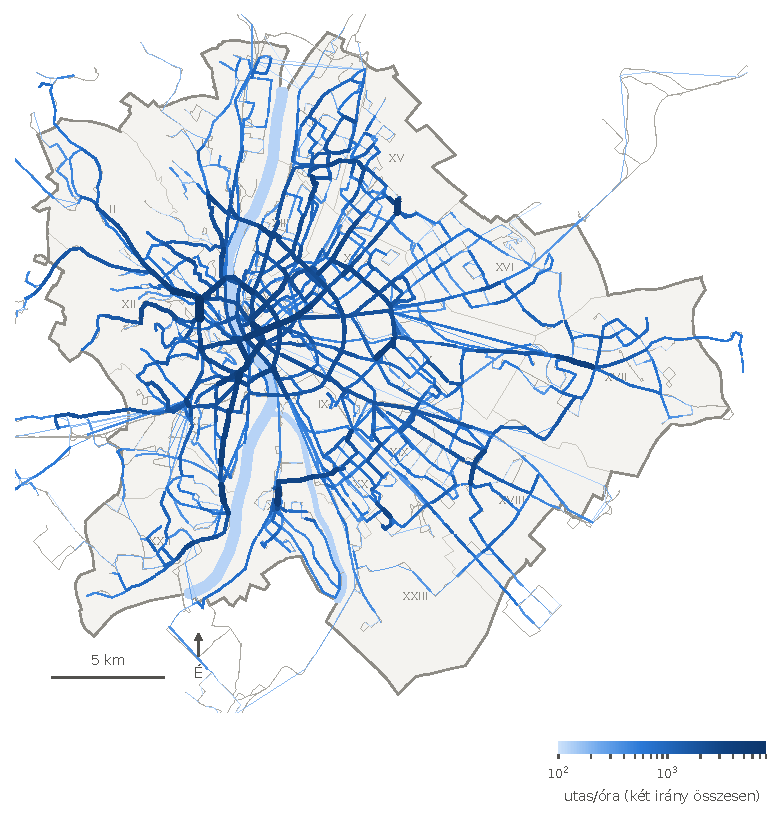
\includegraphics[width=0.93\textwidth]{figures/fig_flow_map.pdf}
  \caption{Stacionárius utasáramlás a reggeli csúcsban (2026.~június~9.,
  07:00--09:00), csomópontpáronként, a két irány és az összes viszonylat
  összegeként. A szürke vonalak a BKK GTFS \texttt{shapes.txt} valós
  útvonalai, a kék sáv a Duna, a vékony körvonalak a kerülethatárok
  (EOV-vetület).}
  \label{fig:flow}
\end{figure}

A legforgalmasabb csomópontok sorrendje (Örs vezér tere, Széll Kálmán tér,
Keleti pályaudvar, Móricz Zsigmond körtér, Kelenföld vasútállomás, Deák
Ferenc tér) megfelel a budapesti átszállóközpontok ismert szerepének. A
legnagyobb, \MAXHUBBOARD{} utas/óra felszállás az Örs vezér terén
adódott. A \ref{tet:poisson}.~tétel szerint a várakozók száma minden
csomópontban Poisson-eloszlású, így a relatív szórás a forgalmas
csomópontokon is $15$--$30\%$, ami a peronméretezésnél nem hanyagolható el.

\paragraph{A modális megoszlás mint ellenőrzés.}
A felszállások \MSBBUS\%-a busz, \MSBTRAM\%-a villamos, \MSBTROLLEY\%-a
trolibusz, \MSBHEV\%-a HÉV és csak \MSBMETRO\%-a metró. A metró
részesedése nagyságrenddel kisebb a valóságosnál. Ez a modell legfontosabb
korlátjára mutat rá: az indulásokkal arányos kiinduló igény a sűrű
buszhálózatra teríti az utasokat, a véletlen bolyongás pedig nem tereli a
hosszú utazásokat a gyors gerincvonalakra. A térbeli \emph{sorrend} ettől még
értelmes, az abszolút szinteket viszont csak igénymátrixszal vagy utasszámláló
adatokkal lehetne kalibrálni (\ref{sec:korlat}.~fejezet).

\subsection{Ellenőrzés és tranziens}

A \ref{tet:poisson}.~tételt független utasok egzakt (Doob--Gillespie)
szimulációjával \citep{gillespie1977} ellenőriztük. \MCN{} szimulált utazás (\MCSEC~s) átlagos
hossza \MCMEAN{} perc (standard hiba \MCSE{} perc), az egzakt érték
\EJOURNEYTWO{} perc, az eltérés \MCRELERR\%. Az $L_x>1$ állapotokban a
foglaltság medián relatív eltérése \MCOCCERR\%, ami a mintaméretből adódó
Monte-Carlo-szórás nagyságrendje. Az utazási idő eloszlása erősen ferde: a
medián \JQFIFTY{}, a $90\%$-os kvantilis \JQNINETY{} perc.

Az üres hálózatból induló feltöltődést a \ref{fig:transient}.~ábra
mutatja. Az átlagos összes foglaltság \TFIFTY{} perc alatt éri el
stacionárius értékének felét, és \TNINETYFIVE{} perc alatt a $95\%$-át. A $T$
spektrális abszcisszájából számolt relaxációs idő viszont \TRELAX{} perc,
mert a leglassabb sajátvektor egy olyan peremkerületi megállóban
lokalizálódik, ahonnan az ablakban egyetlen járat indul (\NSINGLE{}
szakasznak csak egy indulása van). A spektrális rés tehát a legrosszabbul
kiszolgált sarkot jellemzi, nem a rendszer egészét; ugyanez érvényes a
spektrumból számolt globális mutatókra (pl.\ a Kemény-állandóra,
\citealp{kemeny1976}) is. Ezért a sérülékenységet nem spektrális mutatóval
mérjük.

\begin{figure}[!htbp]
  \centering
  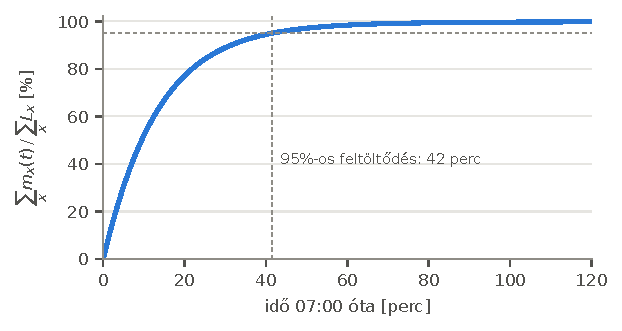
\includegraphics[width=0.62\textwidth]{figures/fig_transient.pdf}
  \caption{Az átlagos összes foglaltság feltöltődése üres kezdőállapotból,
  a \eqref{eq:mt} képlet szerint.}
  \label{fig:transient}
\end{figure}

\paragraph{Érzékenység.}
A $\lambda$, $D$ és $p_{\mathrm{tr}}$ paramétereket egyenként változtattuk.
$\lambda=0$ (tiszta gyakorisági megosztás) esetén az átlagos utazási idő
\SLAMZEROJ{}, $\lambda=1/60$~s$^{-1}$ esetén \SLAMSIXTYJ{} perc, a várakozók
aránya pedig \SLAMZEROW\%-ról \SLAMSIXTYW\%-ra nő, mert az erősebb preferencia
több jármű elutasításával jár. $D=2{,}5$, illetve $5$~km mellett az
utazási idő \SDLOW, illetve \SDHIGH{} perc, $p_{\mathrm{tr}}=0{,}2$,
illetve $0{,}4$ mellett \SPLOW, illetve \SPHIGH{} perc. A térbeli mintázat
ugyanakkor robusztus: a csomóponti felszállások Spearman-féle
rangkorrelációja az alapesettel minden változatban legalább \SMINRHOHUB, a
szakaszterheléseké legalább \SMINRHOSEG.

\subsection{Sérülékenység}

Az ép hálózat igényekkel súlyozott hatékonysága
$E=\EZERO\cdot10^{-4}$~s$^{-1}$, ami \EHARM{} perces harmonikus átlagos
eljutási időnek felel meg. A $60$ legnagyobb forgalmú csomópont bezárását és
megszakadását pontosan kiszámoltuk ($120$ forgatókönyv, \RESSEC{} perc).
A \ref{fig:critical}.~ábra és a \ref{tab:critical}.~táblázat a
hálózati hatás szerinti tíz legkritikusabb csomópontot mutatja.

\begin{figure}[!htbp]
  \centering
  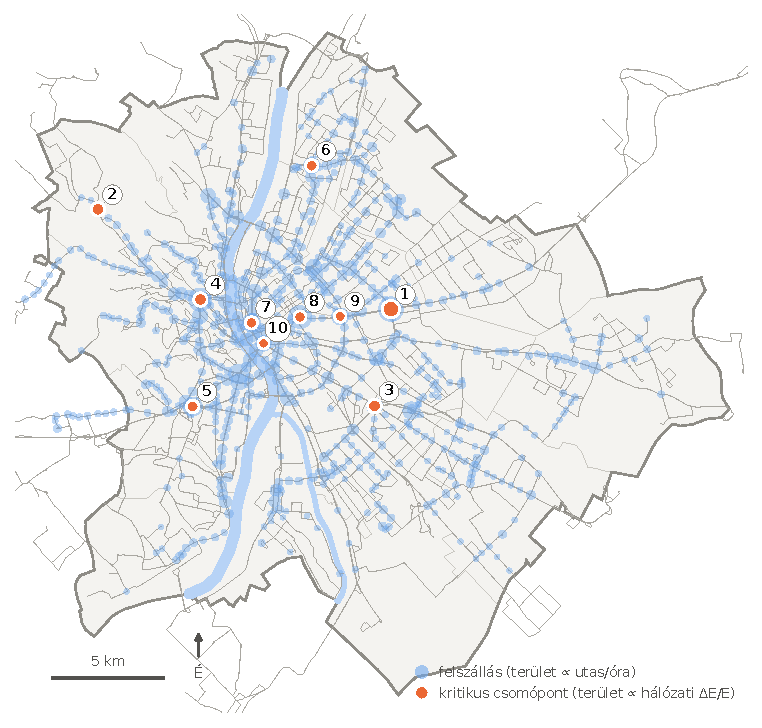
\includegraphics[width=0.93\textwidth]{figures/fig_critical_map.pdf}
  \caption{Csomóponti felszállások (kék) és a bezárás hálózati hatása szerinti
  tíz legkritikusabb csomópont (narancs, a számozás a
  \ref{tab:critical}.~táblázat sorrendje).}
  \label{fig:critical}
\end{figure}

\begin{table}[!htbp]
\centering
\caption{A bezárás hálózati hatása szerinti tíz legkritikusabb csomópont.
Módok: V villamos, M metró, B busz, T trolibusz, H HÉV. $\Delta E/E$:
teljes veszteség; \enquote{hálózati}: a csomópontot nem érintő
utazások hatékonyságvesztesége.}
\label{tab:critical}
\small
\setlength{\tabcolsep}{4.5pt}
\begin{tabular}{rllrrrr}
\toprule
 & & & Felszállás & \multicolumn{2}{c}{Bezárás [\%]} & Megszakadás [\%] \\
\cmidrule(lr){5-6}\cmidrule(lr){7-7}
\# & Csomópont & Mód & [utas/óra] & $\Delta E/E$ & hálózati & hálózati \\
\midrule
\csname @@input\endcsname generated/table_critical.tex
\bottomrule
\end{tabular}
\end{table}

Három megfigyelés emelhető ki. (i) Az Örs vezér tere kiugró: bezárása a
többi utazás hatékonyságát is $3{,}2\%$-kal rontja, mert itt csatlakozik a
gödöllői HÉV, az M2 és a keleti busz- és villamoshálózat. (ii) A hálózati
hatás nem azonos a forgalommal: a rangkorreláció csak \RHOTHRU. A
Hűvösvölgy és a Határ út forgalma közepes, mégis a második és harmadik
helyen áll, mert a budai hegyvidék, illetve a dél-pesti buszhálózat felé
egyetlen átszállási pontként működik. A Deák Ferenc tér ezzel szemben
nagy közvetlen veszteséget okoz, de a párhuzamos metróvonalak és a Kálvin tér
miatt hálózati szerepe kisebb. (iii) Megszakadáskor, amikor a vonalak is
kettészakadnak, a belső metrócsomópontok kerülnek előre
(\FAILNAMEA{} \FAILNETA\%, \FAILNAMEB{} \FAILNETB\%, \FAILNAMEC{}
\FAILNETC\%); a két forgatókönyv rangkorrelációja \RHOCF. A bezárás és a
megszakadás tehát két különböző kérdésre felel: az előbbi az
átszállóközpontok, az utóbbi a pályahálózat sérülékenységét méri.

% =============================================================================
\section{Korlátok}
\label{sec:korlat}

\begin{itemize}
  \item \textbf{Igény.} A kiinduló igény az indulásokkal arányos. Népességi,
    munkahelyi vagy jegyadatok nélkül az abszolút szintek, és különösen a
    módok közötti megoszlás, csak szemléltető jellegűek. A lineáris szerkezet miatt
    a teljes skála egyetlen szorzóban van, a térbeli mintázat viszont csak
    igénymátrixszal kalibrálható.
  \item \textbf{Célirányos útvonalválasztás hiánya.} Az utas nem egy
    célállomás felé halad, hanem csomópontonként választ. A célt is tartalmazó
    állapottér ($\Xs\times\Hs$) elvileg kezelhető, de kalibrálásához
    származási--célállomási adatok kellenek.
  \item \textbf{Kapacitás.} A modell lineáris, azaz nem számol a járművek
    befogadóképességével; zsúfoltságtól függő ráták mellett elveszne a
    Poisson-tétel.
  \item \textbf{Exponenciális tartózkodási idők.} A momentumillesztés csak az
    átlagot illeszti. Erlang-fázisokkal a szórás is illeszthető lenne,
    az állapottér növelése árán; a \ref{tet:poisson}.~tétel ekkor is érvényes.
  \item \textbf{Időbeli homogenitás.} Az ablakon belül állandó rátákat
    feltételezünk. Szakaszonként állandó $T(t)$ mellett a tétel ugyanígy
    érvényes, $e^{Tt}$ helyett időrendezett szorzattal.
  \item \textbf{Sérülékenységi mutató.} A legrövidebb várható idők
    determinisztikus útvonalakat feltételeznek, és egy-egy viszonylat
    várakozási idejével számolnak, ami felülbecsli a több közös vonallal
    kiszolgált párok eljutási idejét.
\end{itemize}

% =============================================================================
\section{Összefoglalás}
\label{sec:osszefoglalas}

A dolgozatban kizárólag nyilvános menetrendi adatokból építettünk
utasáramlási modellt a budapesti közösségi közlekedésre. A vonalszintű nyílt
Markov-hálózatban az utas a járművön marad, amíg le nem száll, a beszállási
ráta a követési idő első két momentumához illeszkedik, a viszonylatválasztás a
minimális relatív entrópia elvéből következik, és Poisson-ritkítással pontosan
megvalósul. A modell egzakt megoldása (független Poisson-foglaltság,
fázistípusú utazási idő) fölöslegessé teszi a sztochasztikus szimulációt,
amelyet csak ellenőrzésre használtunk. A kutatási kérdés három részére tehát
igenlő a válasz: a modell következetes, a teljes hálózaton percek alatt
egzaktul megoldható, és értelmezhető sérülékenységi rangsort ad.

A 2026.~június~9-i reggeli csúcsra a modell a budapesti átszállóközpontok
ismert sorrendjét adja, és rámutat, hogy egy csomópont kritikussága nem
azonos a forgalmával: a Hűvösvölgy vagy a Határ út hálózati szerepe nagyobb,
mint amit forgalmuk sejtetne. A modális megoszlás ugyanakkor világosan jelzi
a következő lépést: az igényoldali adatok bevonását. Mivel a modell lineáris
és egzakt, ez a kalibráció egyszerű: utasszámláló adatok esetén az $\bm L$
és az áramlások lineárisak a $\lambda_h$ forrásokban, így a forrásvektor
nemnegatív legkisebb négyzetes feladattal becsülhető.

\paragraph{Adatok és kód.}
A menetrend: BKK GTFS \FEEDVER{} (CC0), a MobilityData tükréről.
Kerülethatárok: geoBoundaries HUN ADM2 \citep{runfola2020}. A
megvalósítást és a reprodukálás lépéseit az \ref{app:repro}.~függelék írja le.

% =============================================================================
\renewcommand{\refname}{Irodalomjegyzék}
\begin{thebibliography}{99}
\setlength{\itemsep}{2pt}
\small

\bibitem[BKK(2024)]{bkk2024}
Budapesti Közlekedési Központ (2024).
\emph{BUDAPESTREND -- Mobility Report 2024}.
BKK Zrt., Budapest. \url{https://bkk.hu/downloads/33386/}
(letöltve: 2026.~október~4.).

\bibitem[Berman és Plemmons(1994)]{berman1994}
Berman, A., Plemmons, R.~J. (1994).
\emph{Nonnegative Matrices in the Mathematical Sciences}.
SIAM, Philadelphia.

\bibitem[Cats és Jenelius(2014)]{cats2014}
Cats, O., Jenelius, E. (2014).
Dynamic vulnerability analysis of public transport networks: mitigation
effects of real-time information.
\emph{Networks and Spatial Economics}, 14(3--4):435--463.

\bibitem[Chriqui és Robillard(1975)]{chriqui1975}
Chriqui, C., Robillard, P. (1975).
Common bus lines.
\emph{Transportation Science}, 9(2):115--121.

\bibitem[Gillespie(1977)]{gillespie1977}
Gillespie, D.~T. (1977).
Exact stochastic simulation of coupled chemical reactions.
\emph{Journal of Physical Chemistry}, 81(25):2340--2361.

\bibitem[Jackson(1957)]{jackson1957}
Jackson, J.~R. (1957).
Networks of waiting lines.
\emph{Operations Research}, 5(4):518--521.

\bibitem[Jahnke és Huisinga(2007)]{jahnke2007}
Jahnke, T., Huisinga, W. (2007).
Solving the chemical master equation for monomolecular reaction systems
analytically.
\emph{Journal of Mathematical Biology}, 54(1):1--26.

\bibitem[Kemeny és Snell(1976)]{kemeny1976}
Kemeny, J.~G., Snell, J.~L. (1976).
\emph{Finite Markov Chains}.
Springer, New York.

\bibitem[Kingman(1993)]{kingman1993}
Kingman, J.~F.~C. (1993).
\emph{Poisson Processes}.
Oxford University Press, Oxford.

\bibitem[Larson és Odoni(1981)]{larson1981}
Larson, R.~C., Odoni, A.~R. (1981).
\emph{Urban Operations Research}.
Prentice-Hall, Englewood Cliffs.

\bibitem[Latora és Marchiori(2001)]{latora2001}
Latora, V., Marchiori, M. (2001).
Efficient behavior of small-world networks.
\emph{Physical Review Letters}, 87(19):198701.

\bibitem[Neuts(1981)]{neuts1981}
Neuts, M.~F. (1981).
\emph{Matrix-Geometric Solutions in Stochastic Models: An Algorithmic
Approach}.
Johns Hopkins University Press, Baltimore.

\bibitem[Norris(1997)]{norris1997}
Norris, J.~R. (1997).
\emph{Markov Chains}.
Cambridge University Press, Cambridge.

\bibitem[Runfola és mtsai(2020)]{runfola2020}
Runfola, D. és mtsai (2020).
geoBoundaries: A global database of political administrative boundaries.
\emph{PLoS ONE}, 15(4):e0231866.

\bibitem[Snickars és Weibull(1977)]{snickars1977}
Snickars, F., Weibull, J.~W. (1977).
A minimum information principle: Theory and practice.
\emph{Regional Science and Urban Economics}, 7(1--2):137--168.

\bibitem[Spiess és Florian(1989)]{spiess1989}
Spiess, H., Florian, M. (1989).
Optimal strategies: A new assignment model for transit networks.
\emph{Transportation Research Part B}, 23(2):83--102.

\bibitem[Wilson(1969)]{wilson1969}
Wilson, A.~G. (1969).
The use of entropy maximising models in the theory of trip distribution,
mode split and route split.
\emph{Journal of Transport Economics and Policy}, 3(1):108--126.

\end{thebibliography}
% =============================================================================
\appendix
\renewcommand{\thesection}{\Alph{section}}
\section{Megvalósítás és reprodukálhatóság}
\label{app:repro}

A modellt a \texttt{bkk-markov-passenger-flow} Python-csomag valósítja meg
(NumPy, SciPy, pandas; a ritka mátrixokat CSR formában tároljuk). A
dolgozat minden száma, ábrája és táblázata az alábbi lépésekkel állítható elő:
\begin{enumerate}
  \item a BKK GTFS-menetrend (\FEEDVER) letöltése a MobilityData tükréről;
  \item \texttt{python scripts/tdk\_analysis.py --date 20260609}
    (stacionárius megoldás, Monte-Carlo-ellenőrzés, érzékenység,
    $120$ sérülékenységi forgatókönyv; kb.\ $15$ perc);
  \item \texttt{python scripts/tdk\_figures.py} (térképek EOV-vetületben);
  \item \texttt{python scripts/tdk\_tex\_numbers.py} (a szövegbeli számok
    és a táblázat generálása).
\end{enumerate}
A számok tehát nem kézzel kerülnek a szövegbe. A megvalósítást automatikus
tesztek ellenőrzik, köztük a részgenerátor szerkezete, Little törvénye, a
tranziens konvergenciája és az egzakt megoldás Monte-Carlo-összevetése.

\section{Nyilatkozat a mesterséges intelligencia használatáról}
\label{app:mi}

A versenyfelhívás előírása szerint ebben a függelékben kell feltüntetni,
milyen eszközöket és milyen célra használt a szerző. A dolgozat jelen
változatának elkészítésében az Anthropic Claude nagy nyelvi modellje
(Claude Code fejlesztői környezetben) a következő feladatokat végezte:
\begin{itemize}
  \item a Python-kód (modell, elemzés, térképek, tesztek) megírása és
    hibakeresése;
  \item a matematikai levezetések és bizonyítások megfogalmazása;
  \item szakirodalmi források és a BKK közzétett adatainak keresése;
  \item a dolgozat szövegének és ábráinak elkészítése.
\end{itemize}
[A szerző kiegészítése: a saját munka pontos leírása (pl.\ a kutatási kérdés
megfogalmazása, a modellválasztás, az eredmények ellenőrzése és értelmezése,
a szöveg átírása), valamint annak megjelölése, mely részek maradtak
mesterséges intelligenciával előállított formában.]

\end{document}
